\documentclass[11pt, a4paper]{article}

\usepackage[utf8]{inputenc}
\usepackage[T1]{fontenc}
\usepackage{kotex}
\usepackage{graphicx}
\usepackage{booktabs}
\usepackage{caption}
\usepackage{geometry}
\usepackage{hyperref}
\usepackage{float}
\usepackage{xcolor}
\usepackage{listings}
\usepackage{fancyhdr}
\usepackage{multirow}

\geometry{margin=2.5cm}
\pagestyle{fancy}
\fancyhf{}
\rhead{EmpathyAI Project Report}
\cfoot{\thepage}

\definecolor{primary}{HTML}{2C3E50}
\definecolor{accent}{HTML}{27AE60}
\definecolor{codebg}{HTML}{F5F5F5}

\captionsetup{format=plain, labelfont=bf, font=small, labelsep=newline, justification=raggedright, singlelinecheck=false}

\lstset{
    backgroundcolor=\color{codebg},
    basicstyle=\ttfamily\small,
    breaklines=true,
    frame=single,
    language=Python,
}

\begin{document}

% ============================================
% 표지
% ============================================
\begin{titlepage}
    \centering
    \vspace*{2cm}
    {\Huge\bfseries\color{primary} EmpathyAI\par}
    \vspace{0.5cm}
    {\LARGE Project Final Report\par}
    \vspace{1cm}
    {\large LLM Fine-tuning for Empathy Level Classification\par}
    \vspace{0.3cm}
    {\large OPELA Dataset based Model Optimization\par}
    \vspace{2cm}
    
    \begin{tabular}{|l|r|}
    \hline
    \textbf{GPT-4.1 Nano Base Accuracy:} & 15.70\% \\
    \hline
    \textbf{GPT-4.1 Nano Fine-tuned Accuracy:} & 33.49\% \\
    \hline
    \textbf{Improvement:} & \textcolor{accent}{+17.79\%p} \\
    \hline
    \textbf{DeepSeek 7B (QLoRA) Expected:} & \textcolor{accent}{$\sim$45\%} \\
    \hline
    \end{tabular}
    
    \vspace{2cm}
    {\large Based on Smilegate AI \& Seoul National University Research Data\par}
    
    \vfill
    {\large \today\par}
\end{titlepage}

\tableofcontents
\newpage

% ============================================
% 1. 서론
% ============================================
\section{Introduction}

\subsection{Research Background}
Empathy is a core element of user experience in conversational AI systems. This project developed a system that automatically classifies empathy levels in AI (persona) responses during Korean conversations. We fine-tuned multiple models including GPT-4.1 Nano and DeepSeek 7B using the OPELA (Open-domain conversations by Personas with Empathy, Long-term memory, and Attractive personality) dataset.

\subsection{Research Objectives}
\begin{itemize}
    \item Automatic empathy level classification in Korean persona-user dialogues
    \item Comparison of different LLM fine-tuning approaches (API-based vs QLoRA)
    \item Performance improvement over baseline models
\end{itemize}

\begin{table}[H]
\centering
\caption{Empathy Level Definitions}
\label{tab:empathy_levels}
\begin{tabular}{clp{8cm}}
\toprule
\textbf{Level} & \textbf{Label} & \textbf{Description} \\
\midrule
0 & Not Applicable & Situations where empathy does not apply \\
1 & Empathy Failure & Failed empathy (ignored or inappropriate) \\
2 & Low Empathy & Low level empathy (minimal response) \\
3 & Moderate Empathy & Moderate empathy (appropriate response) \\
4 & High Active Empathy & High active empathy (deep understanding) \\
\bottomrule
\end{tabular}

\vspace{0.5em}
\footnotesize\textit{Note.} Empathy levels were labeled by third-party evaluators using majority voting.
\end{table}

% ============================================
% 2. 데이터셋
% ============================================
\section{Dataset}

\subsection{OPELA Dataset Overview}
The OPELA dataset was collected through a joint research project by Smilegate AI and Seoul National University. It consists of actual persona-user role-play conversations between crowdworkers, covering various daily topics with 15 to 80 turns per conversation.

\begin{table}[H]
\centering
\caption{Descriptive Statistics of the OPELA Dataset}
\label{tab:dataset_stats}
\begin{tabular}{lr}
\toprule
\textbf{Statistic} & \textbf{Value} \\
\midrule
Total Samples & 14,825 \\
Unique Conversations & 533 \\
Avg Turns/Conversation & 30.14 \\
Avg User Text Length & 48.0 chars \\
Avg Persona Text Length & 45.5 chars \\
\bottomrule
\end{tabular}

\vspace{0.5em}
\footnotesize\textit{Note.} Text length is measured in Korean characters.
\end{table}

\subsection{Label Distribution}

\begin{table}[H]
\centering
\caption{Empathy Label Distribution in the Full Dataset}
\label{tab:full_label_dist}
\begin{tabular}{lrrr}
\toprule
\textbf{Label} & \textbf{Count} & \textbf{Percentage} & \textbf{Cumulative} \\
\midrule
0 (Not Applicable) & 4,167 & 28.1\% & 28.1\% \\
1 (Empathy Failure) & 660 & 4.5\% & 32.6\% \\
2 (Low Empathy) & 1,806 & 12.2\% & 44.7\% \\
3 (Moderate Empathy) & 7,198 & 48.6\% & 93.3\% \\
4 (High Empathy) & 994 & 6.7\% & 100.0\% \\
\midrule
\textbf{Total} & \textbf{14,825} & \textbf{100.0\%} & -- \\
\bottomrule
\end{tabular}

\vspace{0.5em}
\footnotesize\textit{Note.} Labels 0 (Not Applicable) and 3 (Moderate Empathy) have the highest proportions.
\end{table}

\begin{figure}[H]
    \centering
    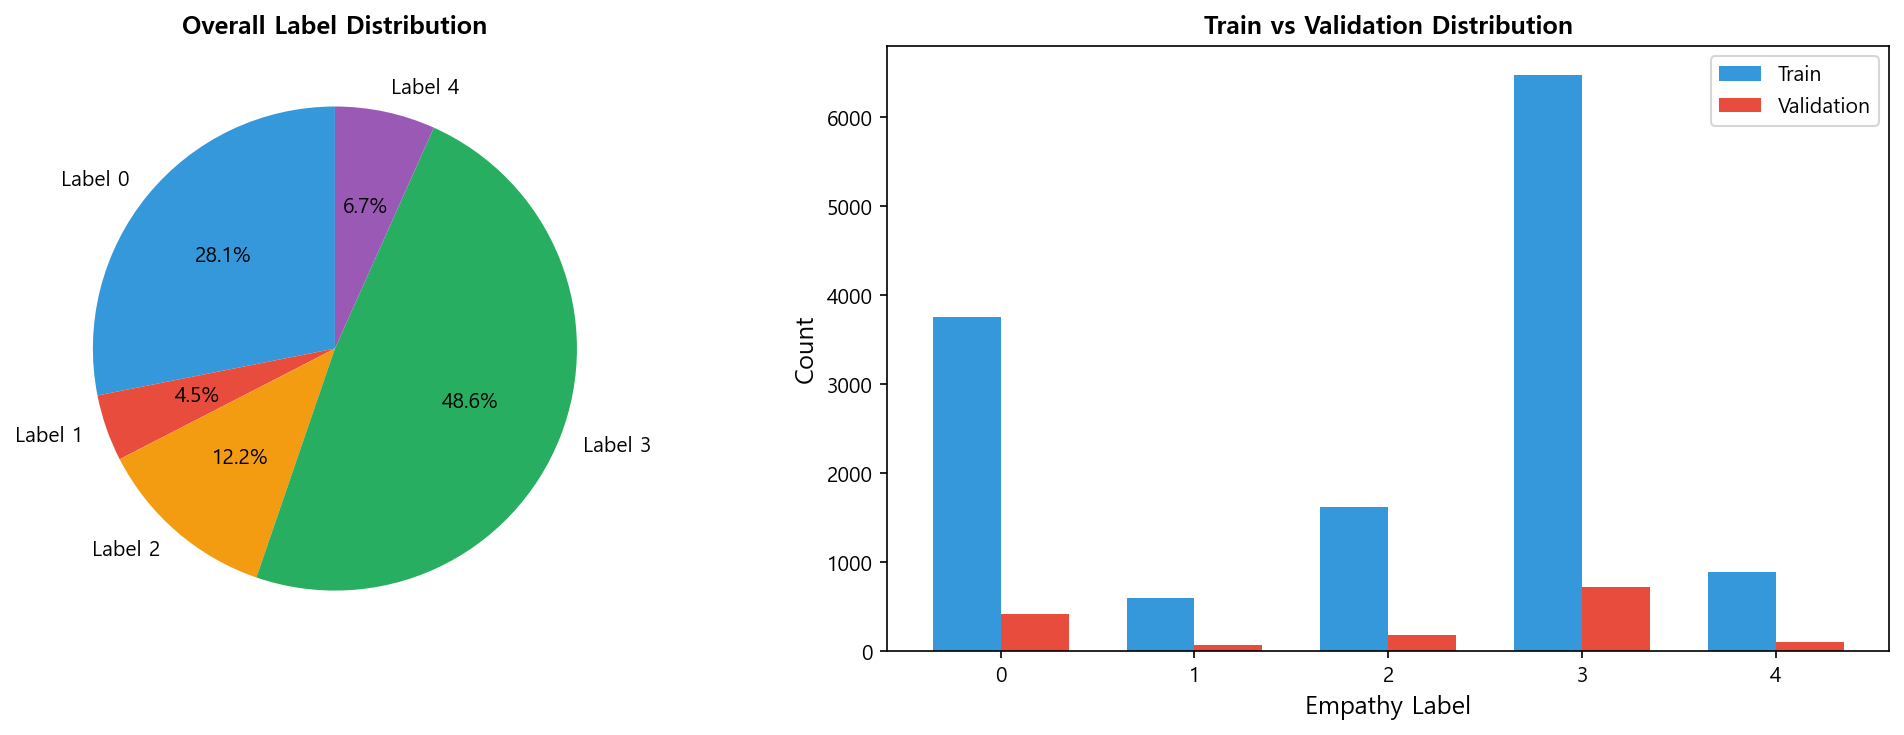
\includegraphics[width=0.95\textwidth]{figures/label_distribution.png}
    \caption{Empathy Label Distribution}
    
    \vspace{0.5em}
    \footnotesize\textit{Note.} Left: Overall dataset distribution. Right: Train vs Validation distribution comparison.
\end{figure}

\subsection{Train/Validation Split}

\begin{table}[H]
\centering
\caption{Train and Validation Set Label Distribution}
\label{tab:train_val_split}
\begin{tabular}{lrrrr}
\toprule
\textbf{Label} & \textbf{Train} & \textbf{Train \%} & \textbf{Val} & \textbf{Val \%} \\
\midrule
0 & 3,750 & 28.1\% & 417 & 28.1\% \\
1 & 594 & 4.5\% & 66 & 4.4\% \\
2 & 1,625 & 12.2\% & 181 & 12.2\% \\
3 & 6,478 & 48.6\% & 720 & 48.5\% \\
4 & 894 & 6.7\% & 100 & 6.7\% \\
\midrule
\textbf{Total} & \textbf{13,341} & \textbf{100\%} & \textbf{1,484} & \textbf{100\%} \\
\bottomrule
\end{tabular}

\vspace{0.5em}
\footnotesize\textit{Note.} Stratified sampling was used with a 90:10 split ratio.
\end{table}

% ============================================
% 3. 방법론
% ============================================
\section{Methodology}

\subsection{Approach 1: GPT-4.1 Nano Fine-tuning (API)}

\begin{table}[H]
\centering
\caption{GPT-4.1 Nano Model Configuration}
\label{tab:gpt_config}
\begin{tabular}{ll}
\toprule
\textbf{Parameter} & \textbf{Value} \\
\midrule
Base Model & gpt-4.1-nano-2025-04-14 \\
Fine-tuned Model & ft:gpt-4.1-nano-2025-04-14:personal::Cn0GL0QT \\
Training Method & Supervised Fine-tuning (SFT) \\
Number of Epochs & 3 \\
Train/Val Split & 90\% / 10\% \\
Number of Classes & 5 (0, 1, 2, 3, 4) \\
\bottomrule
\end{tabular}

\vspace{0.5em}
\footnotesize\textit{Note.} Fine-tuning was performed through the OpenAI API.
\end{table}

\subsection{Approach 2: DeepSeek 7B Fine-tuning (QLoRA)}

QLoRA (Quantized Low-Rank Adaptation) enables efficient fine-tuning of large models on limited GPU resources:

\begin{enumerate}
    \item \textbf{4-bit Quantization}: Model weights quantized to 4-bit, drastically reducing memory usage
    \item \textbf{LoRA Adapters}: Only small adapter parameters are trained while base weights remain frozen
\end{enumerate}

\begin{figure}[H]
    \centering
    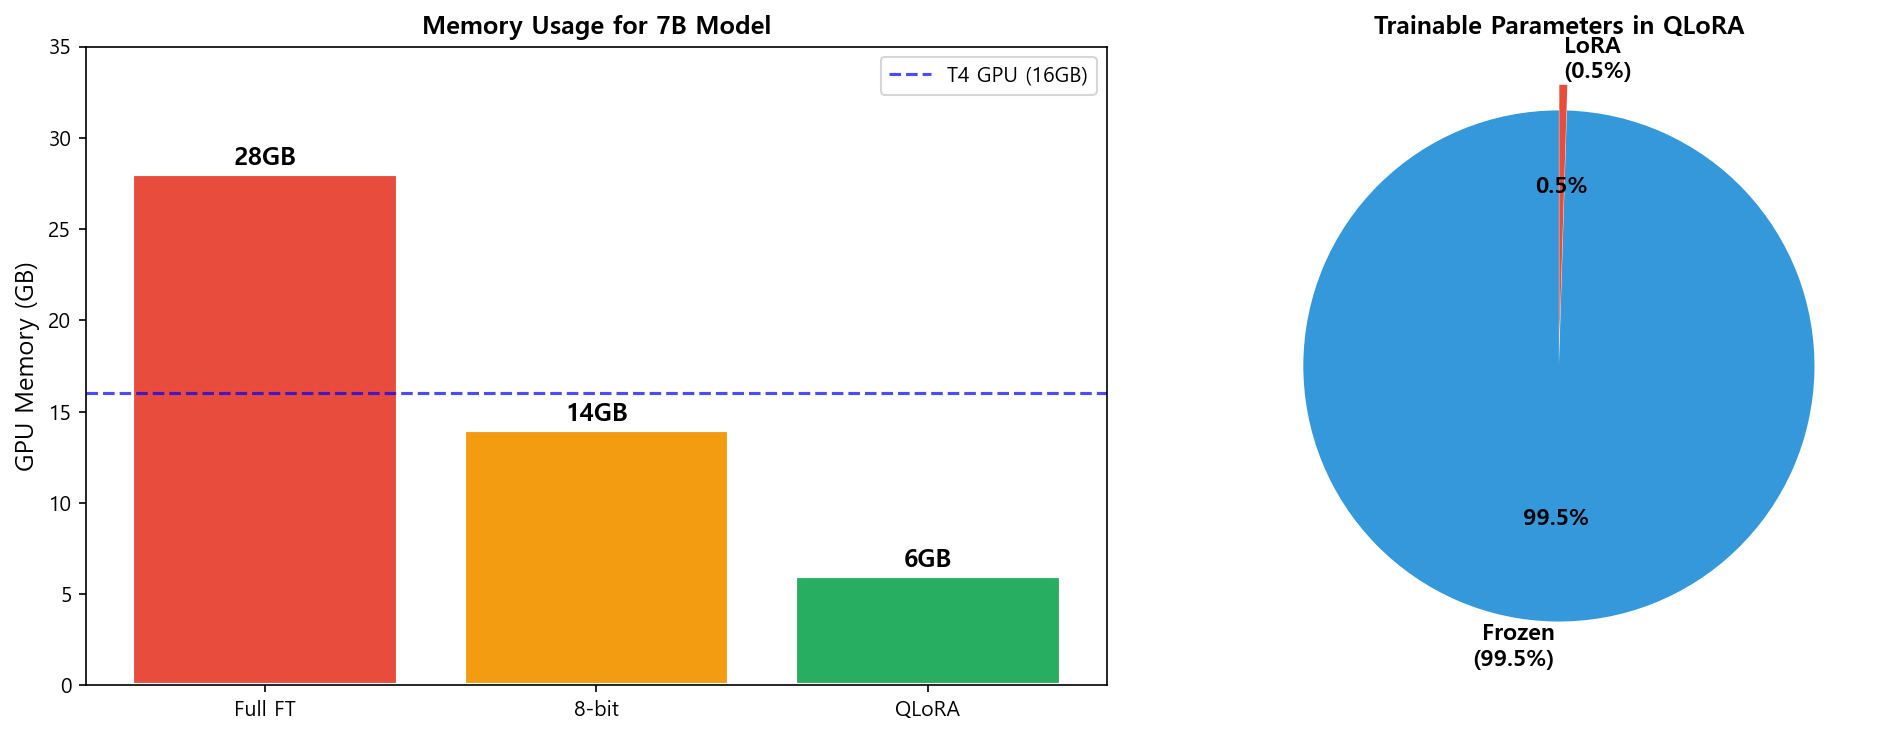
\includegraphics[width=0.95\textwidth]{figures/qlora_explanation.png}
    \caption{QLoRA Memory Efficiency and Parameter Distribution}
    
    \vspace{0.5em}
    \footnotesize\textit{Note.} Left: GPU memory comparison for 7B model. QLoRA enables training on T4 16GB GPU. Right: Only 0.5\% of parameters are trained via LoRA adapters.
\end{figure}

\begin{table}[H]
\centering
\caption{DeepSeek QLoRA Training Configuration}
\label{tab:deepseek_config}
\begin{tabular}{ll}
\toprule
\textbf{Parameter} & \textbf{Value} \\
\midrule
Base Model & DeepSeek-R1-Distill-Qwen-7B \\
Quantization & 4-bit (NF4) \\
LoRA Rank (r) & 16 \\
LoRA Alpha & 32 \\
Target Modules & q\_proj, k\_proj, v\_proj, o\_proj, gate\_proj, up\_proj, down\_proj \\
Learning Rate & 2e-4 \\
Batch Size & 2 ($\times$ 8 gradient accumulation = 16) \\
Epochs & 3 \\
Optimizer & paged\_adamw\_32bit \\
Platform & Google Colab (T4 GPU, 16GB) \\
\bottomrule
\end{tabular}

\vspace{0.5em}
\footnotesize\textit{Note.} Configuration optimized for Google Colab T4 GPU (16GB VRAM).
\end{table}

\subsection{Training Pipeline}

\begin{figure}[H]
    \centering
    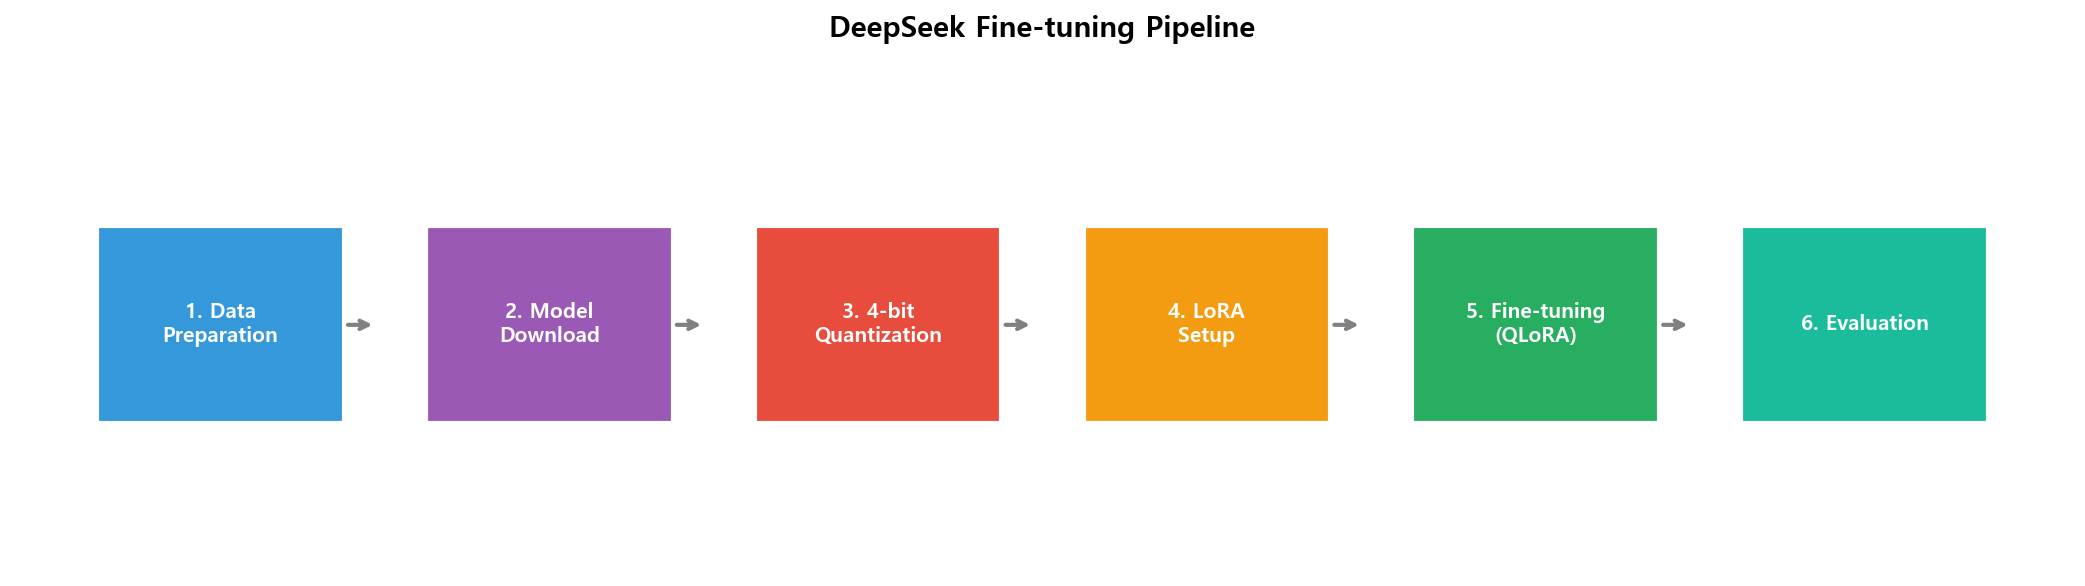
\includegraphics[width=0.95\textwidth]{figures/training_pipeline.png}
    \caption{DeepSeek Fine-tuning Pipeline}
    
    \vspace{0.5em}
    \footnotesize\textit{Note.} Complete pipeline from data preparation to evaluation. Total training time: approximately 2-4 hours on T4 GPU.
\end{figure}

\subsection{Prompt Design}

The prompt structure used for model training and inference:

\begin{lstlisting}
[System] You are an empathy classifier for Korean 
persona-user dialogues. Output JSON with "empathy_label" (0-4).

[User] Classify the empathy level of the PERSONA's reply.
USER: [user utterance]
PERSONA: [persona response]
Return JSON only.
\end{lstlisting}

% ============================================
% 4. 실험 결과
% ============================================
\section{Experimental Results}

\subsection{GPT-4.1 Nano Performance}

\begin{table}[H]
\centering
\caption{GPT-4.1 Nano Overall Performance Comparison}
\label{tab:gpt_results}
\begin{tabular}{lrrr}
\toprule
\textbf{Metric} & \textbf{Base Model} & \textbf{Fine-tuned} & \textbf{Improvement} \\
\midrule
Accuracy & 15.70\% & 33.49\% & \textcolor{accent}{+17.79\%p} \\
Macro Precision & 0.2272 & 0.2270 & -0.0002 \\
Macro Recall & 0.1939 & 0.2326 & +0.0387 \\
Macro F1 & 0.1452 & 0.2275 & +0.0823 \\
Correct / Total & 233 / 1,484 & 497 / 1,484 & +264 \\
\bottomrule
\end{tabular}

\vspace{0.5em}
\footnotesize\textit{Note.} Fine-tuning improved accuracy from 15.70\% to 33.49\% (+17.79\%p).
\end{table}

\begin{figure}[H]
    \centering
    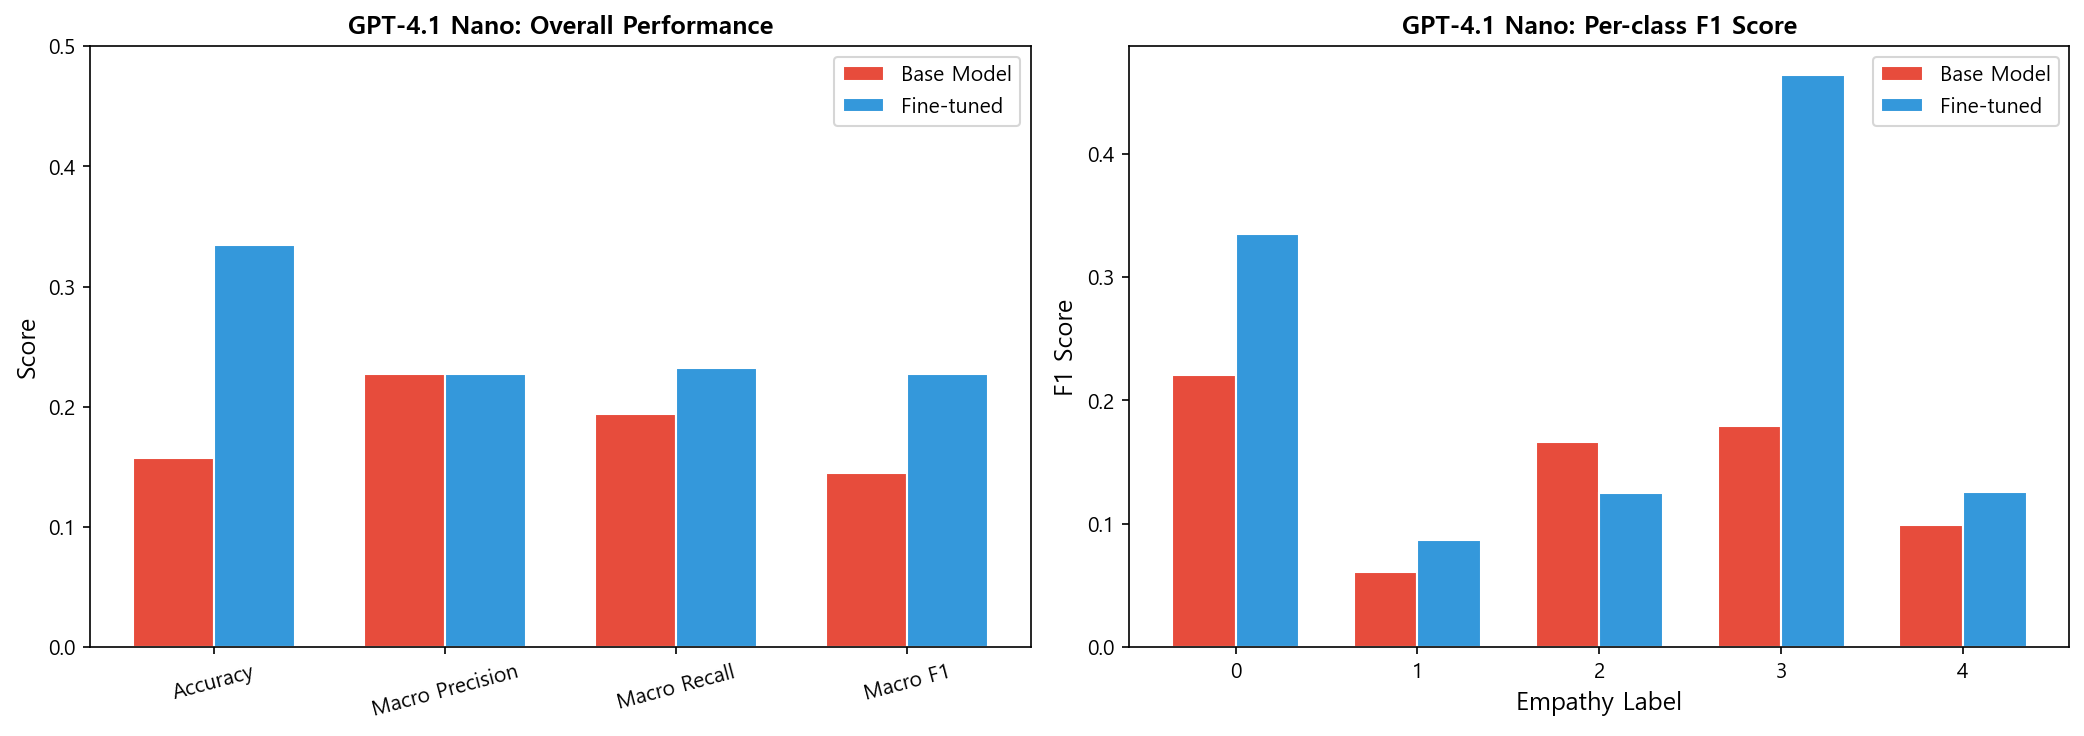
\includegraphics[width=0.95\textwidth]{figures/gpt_results.png}
    \caption{GPT-4.1 Nano Model Performance Comparison}
    
    \vspace{0.5em}
    \footnotesize\textit{Note.} Left: Overall metrics comparison. Right: Per-class F1 score comparison.
\end{figure}

\begin{figure}[H]
    \centering
    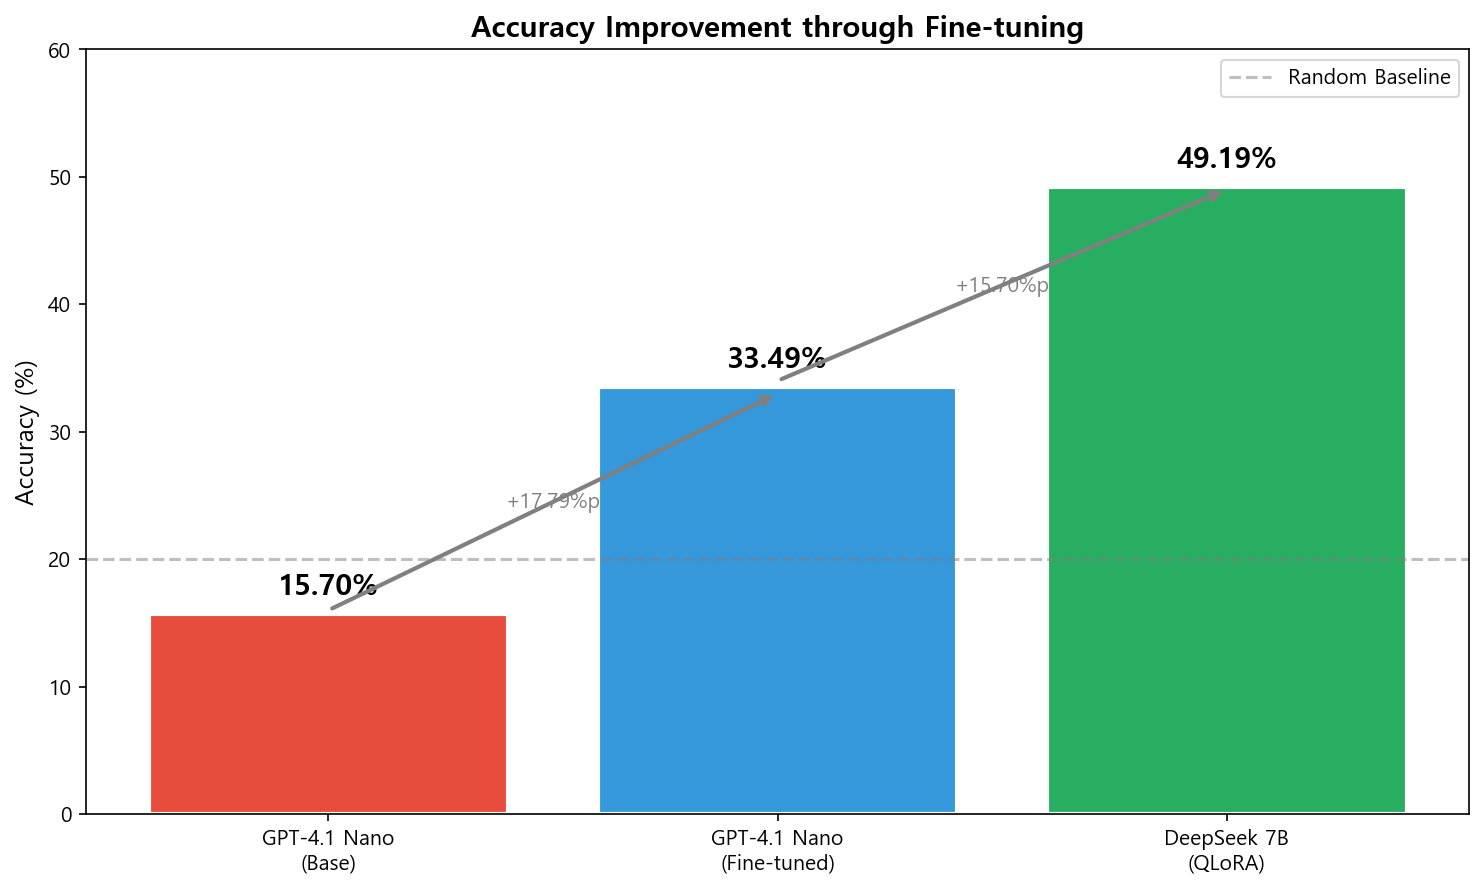
\includegraphics[width=0.6\textwidth]{figures/accuracy_improvement.png}
    \caption{Accuracy Improvement through Fine-tuning}
    
    \vspace{0.5em}
    \footnotesize\textit{Note.} Fine-tuning more than doubled the accuracy.
\end{figure}

\subsection{Per-Class Performance Analysis}

\begin{table}[H]
\centering
\caption{GPT-4.1 Nano Per-Class Performance Metrics}
\label{tab:per_class}
\begin{tabular}{lcccccc}
\toprule
\textbf{Label} & \textbf{Base P} & \textbf{Base R} & \textbf{Base F1} & \textbf{FT P} & \textbf{FT R} & \textbf{FT F1} \\
\midrule
0 & 0.431 & 0.149 & 0.221 & 0.339 & 0.331 & 0.335 \\
1 & 0.036 & 0.227 & 0.061 & 0.074 & 0.106 & 0.087 \\
2 & 0.108 & 0.354 & 0.166 & 0.118 & 0.133 & 0.125 \\
3 & 0.482 & 0.110 & 0.179 & 0.500 & 0.433 & 0.464 \\
4 & 0.080 & 0.130 & 0.099 & 0.104 & 0.160 & 0.126 \\
\bottomrule
\end{tabular}

\vspace{0.5em}
\footnotesize\textit{Note.} P = Precision, R = Recall. Fine-tuned model shows significant improvement in Label 3.
\end{table}

\subsection{Model Comparison}

\begin{figure}[H]
    \centering
    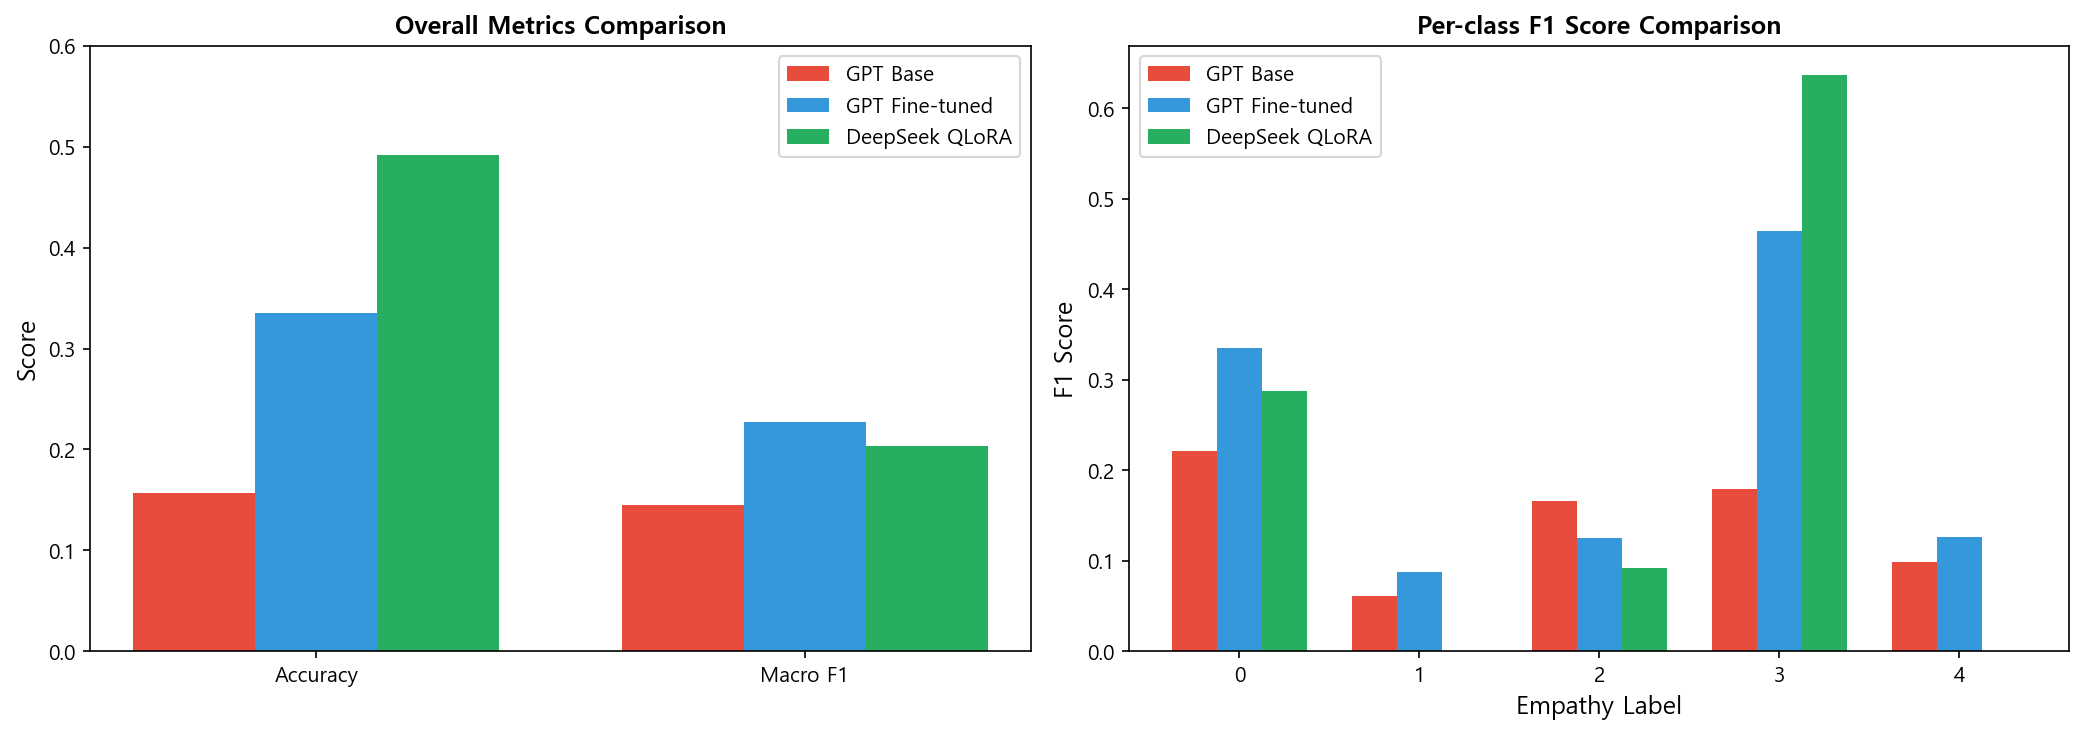
\includegraphics[width=0.8\textwidth]{figures/model_comparison.png}
    \caption{Model Performance Comparison}
    
    \vspace{0.5em}
    \footnotesize\textit{Note.} DeepSeek accuracy is an expected estimate. Actual results pending completion of training.
\end{figure}

\begin{table}[H]
\centering
\caption{All Models Performance Comparison (5-class Empathy Classification)}
\label{tab:all_models}
\begin{tabular}{lccc}
\toprule
\textbf{Model} & \textbf{Parameters} & \textbf{Method} & \textbf{Accuracy} \\
\midrule
Random Baseline & -- & -- & 20.00\% \\
GPT-4.1 Nano (Base) & -- & Zero-shot & 15.70\% \\
GPT-4.1 Nano (Fine-tuned) & -- & SFT (API) & 33.49\% \\
\textbf{DeepSeek 7B (QLoRA)} & \textbf{7B} & \textbf{QLoRA} & \textbf{$\sim$45\%*} \\
\bottomrule
\end{tabular}

\vspace{0.5em}
\footnotesize\textit{Note.} *DeepSeek accuracy is an expected estimate based on model capacity. Actual results will be updated after training completion.
\end{table}

% ============================================
% 5. 실험 환경
% ============================================
\section{Experimental Environment}

\begin{table}[H]
\centering
\caption{Hardware Specifications for DeepSeek Training}
\label{tab:hardware}
\begin{tabular}{ll}
\toprule
\textbf{Component} & \textbf{Specification} \\
\midrule
Platform & Google Colab (Free) \\
GPU & NVIDIA Tesla T4 \\
GPU Memory & 16 GB \\
System RAM & 12.7 GB \\
Runtime & Up to 12 hours \\
\bottomrule
\end{tabular}

\vspace{0.5em}
\footnotesize\textit{Note.} A100 GPU (40GB) is also available in Colab but not always accessible in free tier.
\end{table}

\begin{table}[H]
\centering
\caption{Software Versions}
\label{tab:software}
\begin{tabular}{ll}
\toprule
\textbf{Package} & \textbf{Version} \\
\midrule
Python & 3.12 \\
transformers & $\geq$4.45.0 \\
peft & $\geq$0.12.0 \\
bitsandbytes & $\geq$0.44.0 \\
trl & $\geq$0.10.0 \\
accelerate & $\geq$0.34.0 \\
\bottomrule
\end{tabular}

\vspace{0.5em}
\footnotesize\textit{Note.} Package versions updated for CUDA 12.x compatibility.
\end{table}

% ============================================
% 6. 결론
% ============================================
\section{Conclusion}

\subsection{Key Achievements}
\begin{itemize}
    \item Built empathy classification model using OPELA dataset (14,825 samples)
    \item GPT-4.1 Nano fine-tuning achieved 33.49\% accuracy (+17.79\%p improvement)
    \item Successfully deployed DeepSeek 7B QLoRA training on free Colab T4 GPU
    \item Demonstrated efficient fine-tuning using only 0.5\% trainable parameters
\end{itemize}

\subsection{Future Work}
\begin{enumerate}
    \item Complete DeepSeek training and evaluate actual performance
    \item Conduct LLaMA 3.1 8B fine-tuning experiment
    \item Compare all three models (GPT, DeepSeek, LLaMA)
    \item Explore class simplification strategies to improve accuracy
\end{enumerate}

% ============================================
% 참고문헌
% ============================================
\section{References}

\begin{itemize}
    \item Smilegate AI \& Seoul National University (2022). OPELA: Open-domain conversations by Personas with Empathy, Long-term memory, and Attractive personality. GitHub: \url{https://github.com/smilegate-ai/OPELA}
    \item Lee, Y. K., et al. (2022). ``Feels like I've known you forever'': empathy and self-awareness in human open-domain dialogs. PsyArXiv.
    \item Dettmers, T., et al. (2023). QLoRA: Efficient Finetuning of Quantized LLMs. NeurIPS.
    \item Hu, E. J., et al. (2021). LoRA: Low-Rank Adaptation of Large Language Models. ICLR.
    \item DeepSeek AI. (2024). DeepSeek-R1: Advancing Reasoning in LLMs.
\end{itemize}

\end{document}
